% ***************************************************
% Appendix
% ***************************************************
\chapter{Supplementary information for Chapter 5}

\hypertarget{pama-nyungan-reference-phylogeny}{%
\section{Pama-Nyungan reference
phylogeny}\label{pama-nyungan-reference-phylogeny}}

Quantifying phylogenetic signal requires an independently-derived
reference phylogeny as a yardstick. Our reference phylogeny is a 128-tip
subset of the 285-tip Pama-Nyungan phylogeny presented by
\textcite{bowern_pama-nyungan_2015}, corresponding to the 128 wordlists
used in this study (Figure A.2.1).

\begin{figure}
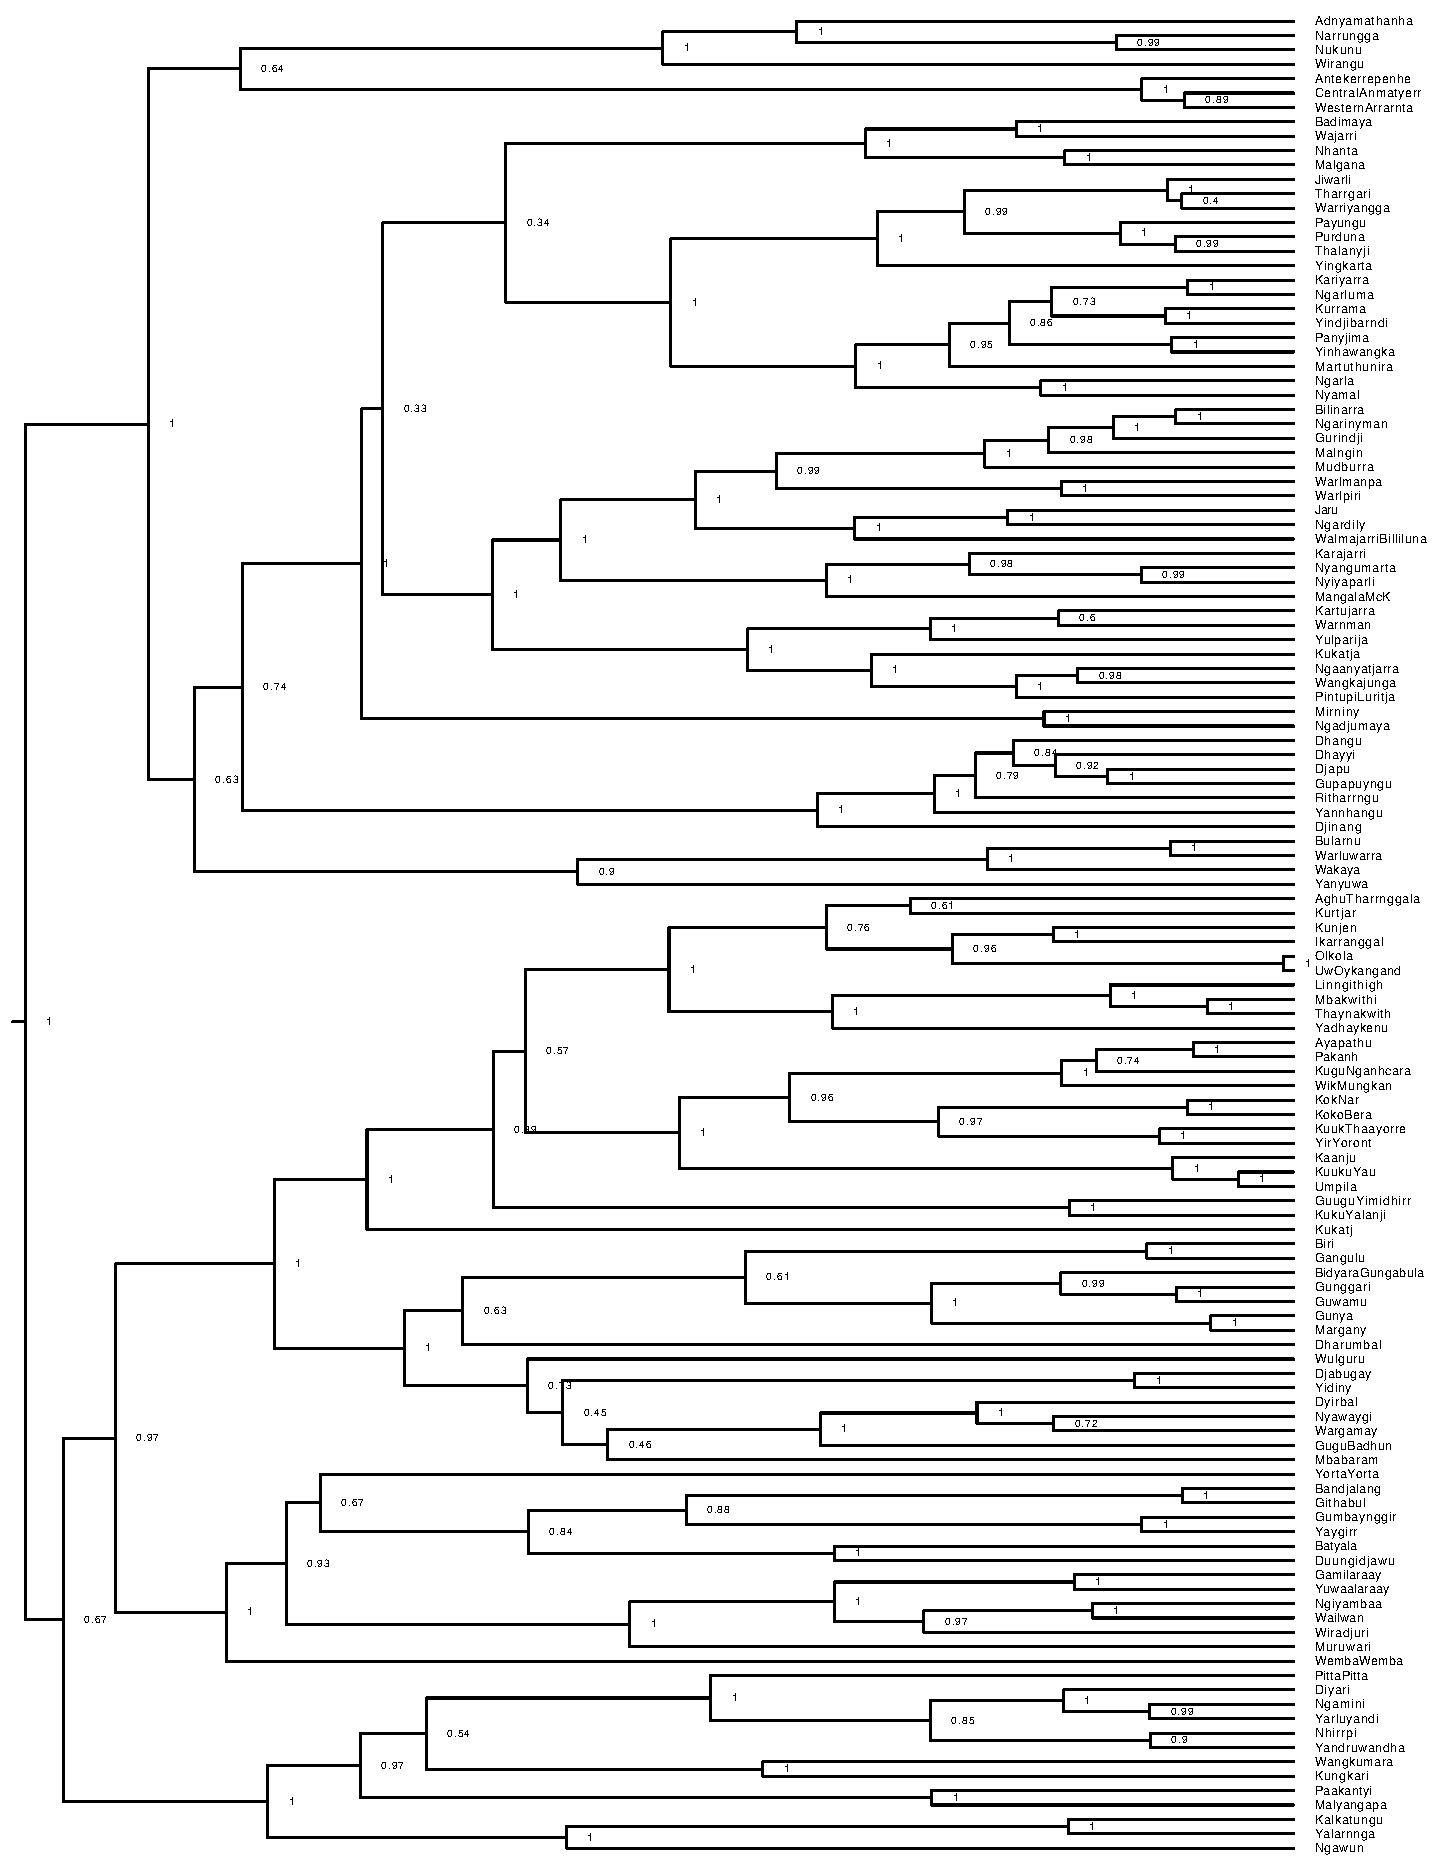
\includegraphics[width=1\linewidth]{Appendix-B/fig/PN_tree_with_posteriors} \caption{Figure A.2.1. Pama-Nyungan reference phylogeny. Posterior probability values from Bowern (2015) have been added, giving an indication of support for each node. Although there is no strict, conventional cut-off, clades with posterior values above 0.5 are considered supported and values above 0.8 are considered strongly supported (Bowern \& Atkinson 2012, p.829).}\label{fig:plot-ref-tree2}
\end{figure}

As discussed in the main paper, the reference phylogeny was constructed
using Bayesian phylogenetic methods in the software BEAST2
\autocite{bouckaert_beast_2014}. Bayesian phylogenetic methods use a
Markov Chain Monte Carlo (MCMC) procedure to efficiently search the
hypothesis space of possible trees and return a large posterior sample
of possibilities (from which an indication of uncertaintly can be
derived). The tree contained in the nexus file above is a maximum clade
credibility tree, which is a summation of the posterior sample of the
\textcite{bowern_pama-nyungan_2015} analysis where the likelihood of all
nodes in the tree (in terms of how frequently a given node reappears
across the posterior sample) is maximized.

For further details on the Pama-Nyungan phylogeny used as a reference
phylogeny in this study, see \textcite{bowern_pama-nyungan_2015}. See
also \textcite{bowern_computational_2012}, which infers a Pama-Nyungan
phylogeny in the same way, using exactly the same evolutionary model
parameters, but with an earlier iteration of the dataset containing
fewer doculects. Additional discussion of the general process of
constructing language phylogenies in BEAST2 can be found in
\textcite{bouckaert_origin_2018}, although a different evolutionary
model is used.

The reference phylogeny was inferred using lexical cognate data, coded
according to the principles of the Comparative Method. The cognate data
used in \textcite{bowern_pama-nyungan_2015} is publicly available on
Zenodo \autocite{bowern_pama-nyungan_2018} and also as a subset of the
305-language dataset in \textcite{bouckaert_origin_2018}. This latter
source also includes a Perl script for converting multistate cognate
judgements into a binary matrix for use with BEAST2 phylogenetic
software and will include information on underlying sources.

\newpage

\hypertarget{wordlist-sources}{%
\section{Wordlist sources}\label{wordlist-sources}}

The 128 wordlists used in this study are contained within the Ausphonlex
database, under development by \textcite{round_ausphon-lexicon_2017}.
All underlying wordlist data is available, either publicly in the
CHIRILA database \autocite{bowern_chirila_2016} or elsewhere in
published or archived form. A list of original sources for all wordlists
is presented below.

\textbf{Adnyamathanha}\\
CHIRILA source: CHIRILA/v2/McEnteeMcKenzie

\fullcite{mcentee_adna-mat-na_1992}

\textbf{Aghu Tharnggala}\\
CHIRILA source: CHIRILA/not\_released/jol89

\fullcite{jolly_aghu_1989}

\textbf{Anguthimri}\\
CHIRILA source: CHIRILA/v1/ASEDA0240

\fullcite{crowley_mbakwithi_1989}

\textbf{Antekerrepenhe}\\
CHIRILA source: CHIRILA/not\_released/ASEDA0112

\fullcite{breen_antekerrepenhe_2006}

\textbf{Ayapathu}\\
CHIRILA source: CHIRILA/v2/Hamilton-web

\fullcite{hamilton_ayapathu_1997}

\textbf{Badimaya}\\
CHIRILA source: CHIRILA/not\_released/ASEDA0615

\fullcite{marmion_badimaya_1995}

\textbf{Bakanh}\\
\fullcite{hamilton_pakanh_1997}

\textbf{Bidyara}\\
CHIRILA source: CHIRILA/not\_released/bre73

\fullcite{breen_bidyara_1973}

\textbf{Bilinarra}\\
\fullcite{meakins_bilinarra_2013}

\textbf{Biri}\\
CHIRILA source: CHIRILA/v1/Terrell

\fullcite{terrill_biri_1999}

\textbf{Bularnu}\\
CHIRILA source: CHIRILA/not\_released/ASEDA0007

\fullcite{breen_bularnu_1988}

\textbf{Butchulla}\\
CHIRILA source: CHIRILA/not\_released/ASEDA0769

\fullcite{bell_sketch_2003}

\textbf{Dhangu}\\
CHIRILA source: CHIRILA/not\_released/Zorc-Pepperill

\fullcite{zorc_yolngu_2004}

\textbf{Dharumbal}\\
CHIRILA source: CHIRILA/v2/ter02

\fullcite{terrill_dharumbal:_2002}

\textbf{Dhay'yi}\\
CHIRILA source: CHIRILA/not\_released/ASEDA0502

\fullcite{wunungmurra_dhalwangu_1993}

\textbf{Diyari}\\
\fullcite{austin_grammar_2011}

\textbf{Djabugay}\\
CHIRILA source: CHIRILA/not\_released/ASEDA0013

\fullcite{robertson_jaabugay_1997}

\textbf{Djapu}\\
CHIRILA source: CHIRILA/v1/mor83

\fullcite{morphy_djapu_1983}

\textbf{Djinang}\\
CHIRILA source: CHIRILA/v1/ASEDA0009

\fullcite{waters_djinang_1988}

\textbf{Duungidjawu}\\
CHIRILA source: CHIRILA/v2/K\&W 04

\fullcite{kite_duungidjawu_2004}

\textbf{Dyirbal}\\
CHIRILA source: CHIRILA/v1/dix72

\fullcite{dixon_dyirbal_1972}

\textbf{Gamilaraay}\\
CHIRILA source: CHIRILA/v1/ash03

\fullcite{ash_gamilaraay_2003}

\textbf{Gangulu}\\
CHIRILA source: CHIRILA/v1/Terrell

\fullcite{terrill_biri_1999}

\textbf{Gidabal}\\
CHIRILA source: CHIRILA/v1/cro78

\fullcite{crowley_middle_1978}

\textbf{Gugu Badhun}\\
CHIRILA source: CHIRILA/v1/sut73

\fullcite{sutton_gugu-badhun_1973}

\textbf{Gumbaynggir}\\
CHIRILA source: CHIRILA/not\_released/gumbay01

\fullcite{murrbay_aboriginal_and_culture_cooperative_gumbaynggir_2001}

\textbf{Gunggari}\\
CHIRILA source: CHIRILA/v1/hol88

\fullcite{holmer_notes_1988}

\textbf{Gunya}\\
CHIRILA source: CHIRILA/v1/dixbla81

\fullcite{breen_margany_1981}

\textbf{Gupapuyngu}\\
CHIRILA source: CHIRILA/v1/BL

\fullcite{lowe_temporary_1976}

\textbf{Gurindji}\\
\fullcite{meakins_gurindji_2013}

\textbf{Guugu Yimidhirr}\\
\fullcite{haviland_guugu_1979}

\textbf{Guwamu}\\
CHIRILA source: CHIRILA/v1/Austin 1980

\fullcite{austin_guwamu_1980}

\textbf{Ikarranggal}\\
CHIRILA source: CHIRILA/not\_released/som99

\textbf{Jaru}\\
CHIRILA source: CHIRILA/not\_released/Tsunoda-ASEDA

\fullcite{tsunoda_jaru_1981}

\textbf{Jiwarli}\\
CHIRILA source: CHIRILA/v2/ASEDA0435

\fullcite{austin_dictionary_nodate-1}

\textbf{Kaantju}\\
\fullcite{sommer_coen_nodate}

\textbf{Kalkatungu}\\
CHIRILA source: CHIRILA/v2/ASEDA0205

\fullcite{blake_kalkatungu_1990}

\textbf{Karajarri}\\
CHIRILA source: CHIRILA/not\_released/ASEDA0069 (McKelson)

\fullcite{mckelson_studies_1989}

\textbf{Kariyarra}\\
CHIRILA source: CHIRILA/not\_released/ASEDA0582

\fullcite{smythe_kariyarra_nodate}

\textbf{Kartujarra}\\
CHIRILA source: CHIRILA/not\_released/ASEDA0067

\fullcite{ogrady_gardudjarra_1988}

\textbf{Kok Nar}\\
\fullcite{sommer_koko_nodate}

\textbf{Koko Bera}\\
CHIRILA source: CHIRILA/not\_released/PBKB

\fullcite{black_kokoberrin_1999}

\textbf{Kugu Nganhcara}\\
CHIRILA source: CHIRILA/v1/ASEDA0021

\fullcite{smith_kugu_1989}

\textbf{Kukatj}\\
CHIRILA source: CHIRILA/not\_released/ASEDA0022

\fullcite{breen_kukatj_1991}

\textbf{Kukatja}\\
CHIRILA source: CHIRILA/v1/ASEDA0504

\fullcite{peile_basic_nodate}

\textbf{Kuku Yalanji}\\
\fullcite{hershberger_kuku-yalanji_1986}

\textbf{Kungkari}\\
CHIRILA source: CHIRILA/v1/bre90

\fullcite{breen_salvage_1990}

\textbf{Kurrama}\\
CHIRILA source: CHIRILA/not\_released/ASEDA0481

\fullcite{dench_kurrama_nodate}

\textbf{Kurtjar}\\
CHIRILA source: CHIRILA/v1/ASEDA0026

\fullcite{black_kurtjar_nodate}

\textbf{Kuugu Ya'u}\\
CHIRILA source: CHIRILA/not\_released/ASEDA0027

\fullcite{thompson_sand_1988}

\textbf{Linngithigh}\\
CHIRILA source: CHIRILA/not\_released/ASEDA0687

\fullcite{hale_linngithigh_1999}

\textbf{Malkana}\\
\fullcite{gargett_salvage_2011}

\textbf{Malngin}\\
\fullcite{ise_grammatical_1999}

\textbf{Malyangapa}\\
CHIRILA source: CHIRILA/not\_released/LH/fn

\textbf{Mangala}\\
CHIRILA source: CHIRILA/not\_released/ASEDA0220

\fullcite{mckelson_mangala_1989}

\textbf{Margany}\\
CHIRILA source: CHIRILA/v1/bre81

\fullcite{breen_margany_1981}

\textbf{Martuthunira}\\
\fullcite{dench_martuthunira_1995}

\textbf{Mbabaram}\\
CHIRILA source: CHIRILA/not\_released/dix91m

\fullcite{dixon_mbabaram_1991}

\textbf{Mirrniny}\\
CHIRILA source: CHIRILA/not\_released/ASEDA0070

\fullcite{ogrady_mirniny_1988}

\textbf{Mudburra}\\
CHIRILA source: CHIRILA/not\_released/ASEDA0031

\fullcite{nash_mudburra_1988}

\textbf{Muruwari}\\
CHIRILA source: CHIRILA/v1/ASEDA0252

\fullcite{oates_muruwari_1992}

\textbf{Narrungga}\\
CHIRILA source: CHIRILA/v1/NharranggaWarra

\fullcite{narungga_aboriginal_progress_association_nharangga_2006}

\textbf{Ngaanyatjarra}\\
\fullcite{glass_ngaanyatjarra_1988}

\textbf{Ngadjunmaya}\\
\fullcite{wangka_maya_pilbara_aboriginal_language_centre_ngajumaya_2008}

\textbf{Ngamini}\\
CHIRILA source: CHIRILA/v1/brendn

\fullcite{breen_ngamini_1975}

\textbf{Ngardily}\\
CHIRILA source: CHIRILA/not\_released/ASEDA0034

\fullcite{green_ngardily_1988}

\textbf{Ngarinyman}\\
CHIRILA source: CHIRILA/not\_released/ASEDA0796

\fullcite{jones_ngarinman_2005}

\textbf{Ngarla}\\
CHIRILA source: CHIRILA/not\_released/ASEDA0060

\fullcite{brown_ngarla-english_nodate}

\textbf{Ngarluma}\\
CHIRILA source: CHIRILA/not\_released/ASEDA0037

\fullcite{hale_ngarluma_1989}

\textbf{Ngawun}\\
CHIRILA source: CHIRILA/v2/BreenMayi

\fullcite{breen_mayi_1981}

\textbf{Ngiyambaa}\\
CHIRILA source: CHIRILA/v1/don-lex

\fullcite{donaldson_ngiyambaa_1997}

\textbf{Nhanda}\\
CHIRILA source: CHIRILA/v1/ble01

\fullcite{blevins_nhanda:_2001}

\textbf{Nhangu}\\
CHIRILA source: CHIRILA/v1/CB-fieldnotes

\fullcite{james_yan-nhangu_2003}

\textbf{Nhirrpi}\\
CHIRILA source: CHIRILA/v1/bow-nhi

\fullcite{bowern_nhirrpi_1999}

\textbf{Nukunu}\\
CHIRILA source: CHIRILA/v2/her92

\fullcite{hercus_nukunu_1992}

\textbf{Nyamal}\\
\fullcite{burgman_nyamal_2007}

\textbf{Nyangumarta}\\
CHIRILA source: CHIRILA/not\_released/ASEDA0217

\fullcite{geytenbeek_nyangumarta-english_1991}

\textbf{Nyawaygi}\\
\fullcite{dixon_nyawaygi_1983}

\textbf{Nyiyaparli}\\
CHIRILA source: CHIRILA/not\_released/ASEDA0074

\fullcite{ogrady_nyiyabali_1988}

\textbf{Ogh Unyjan}\\
\fullcite{sommer_ogh_nodate-1}

\textbf{Olkol}\\
\fullcite{hamilton_uw_1997}

\textbf{Oykangand}\\
\fullcite{hamilton_uw_1997}

\textbf{Panyjima}\\
CHIRILA source: CHIRILA/not\_released/ASEDA0375

\fullcite{dench_panyjima_1991-1}

\textbf{Payungu}\\
CHIRILA source: CHIRILA/v1/ASEDA0394

\fullcite{austin_payungu_nodate}

\textbf{Pintupi}\\
\fullcite{hansen_pintupi/luritja_1992}

\textbf{Pitta Pitta}\\
CHIRILA source: CHIRILA/v1/bla0275

\fullcite{blake_pitta_1990}

\textbf{Purduna}\\
\fullcite{burgman_burduna_2007}

\textbf{Ritharrngu}\\
CHIRILA source: CHIRILA/v1/Heath

\fullcite{heath_ritharngu_1976}

\textbf{Southern Paakintyi}\\
CHIRILA source: CHIRILA/not\_released/ASEDA0525

\fullcite{hercus_paakantyi_nodate}

\textbf{Thaayorre}\\
\fullcite{foote_kuuk_1995}

\textbf{Thalanyji}\\
CHIRILA source: CHIRILA/v2/ASEDA0437

\fullcite{austin_dictionary_nodate-2}

\textbf{Tharrkari}\\
\fullcite{austin_dictionary_1992}

\textbf{Thaynakwithi}\\
\fullcite{fletcher_thanakupis_2007}

\textbf{Umpila}\\
CHIRILA source: CHIRILA/not\_released/ASEDA0094

\fullcite{ogrady_umpila_1988}

\textbf{Waalubal}\\
CHIRILA source: CHIRILA/v1/cro78

\fullcite{crowley_middle_1978}

\textbf{Walmajarri}\\
CHIRILA source: CHIRILA/not\_released/ASEDA0167

\fullcite{hudson_walmajarri_1993}

\textbf{Wangkajunga}\\
CHIRILA source: CHIRILA/not\_released/ASEDA0709

\fullcite{blyth_wangka_2001}

\textbf{Wangkumara}\\
CHIRILA source: CHIRILA/v1/robnd

\fullcite{robertson_wangkumara_1985}

\textbf{Warlmanpa}\\
CHIRILA source: CHIRILA/not\_released/ASEDA0049

\fullcite{nash_preliminary_1984}

\textbf{Warlpiri}\\
CHIRILA source: CHIRILA/v2/WarlpiriDict

\fullcite{schwartz_walpiri_1996}

\textbf{Warluwarra}\\
CHIRILA source: CHIRILA/not\_released/ASEDA0253

\fullcite{breen_warluwara_1990}

\textbf{Warnman}\\
CHIRILA source: CHIRILA/v2/ASEDA0334

\fullcite{eidwun_warnman_nodate}

\textbf{Warrgamay}\\
CHIRILA source: CHIRILA/v1/dixbla81

\fullcite{dixon_wargamay_1981}

\textbf{Warriyangga}\\
CHIRILA source: CHIRILA/not\_released/ASEDA0439

\fullcite{austin_dictionary_nodate-3}

\textbf{Watjarri}\\
\fullcite{mackman_wajarri_2012}

\textbf{Wayilwan}\\
CHIRILA source: CHIRILA/v2/Wail-lex

\fullcite{donaldson_wailwan_nodate}

\textbf{Wemba Wemba}\\
CHIRILA source: CHIRILA/not\_released/herw

\fullcite{hercus_wembawemba_1992}

\textbf{Western Anmatyerre}\\
CHIRILA source: CHIRILA/not\_released/gre03ca

\fullcite{green_central_2003}

\textbf{Western Arrernte}\\
CHIRILA source: CHIRILA/not\_released/bre00

\fullcite{breen_introductory_2000}

\textbf{Western Wakaya}\\
CHIRILA source: CHIRILA/not\_released/ASEDA0047

\fullcite{breen_wakaya_2006}

\textbf{Wik Mungkan}\\
\fullcite{kilham_wik_2011}

\textbf{Wiradjuri}\\
CHIRILA source: CHIRILA/v2/Hosking/McNicol1993

\fullcite{hosking_wiradjuri_1993}

\textbf{Wirangu}\\
CHIRILA source: CHIRILA/not\_released/Her99

\fullcite{hercus_grammar_1999}

\textbf{Wulguru}\\
CHIRILA source: CHIRILA/not\_released/Don07

\fullcite{donohue_wulguru:_2007}

\textbf{Yadhaykenu}\\
\fullcite{crowley_uradhi_1983}

\textbf{Yalarnnga}\\
CHIRILA source: CHIRILA/v1/ASEDA0204

\fullcite{breen_yalarnnga_nodate}

\textbf{Yandruwandha}\\
CHIRILA source: CHIRILA/v1/breyandr

\textbf{Yanyuwa}\\
CHIRILA source: CHIRILA/not\_released/ASEDA0382

\fullcite{bradley_yanyuwa_nodate}

\textbf{Yarluyandi}\\
CHIRILA source: CHIRILA/v1/ASEDA0251

\fullcite{hercus_yarluyandi_nodate}

\textbf{Yaygir}\\
CHIRILA source: CHIRILA/v1/morelli2011

\fullcite{morelli_yaygirr_2012}

\textbf{Yidiny}\\
CHIRILA source: CHIRILA/v2/dix91

\fullcite{dixon_words_1991}

\textbf{Yindjibarndi}\\
CHIRILA source: CHIRILA/not\_released/ASEDA0297

\fullcite{anderson_yindjibarndi_nodate}

\textbf{Yingkarta}\\
CHIRILA source: CHIRILA/not\_released/ASEDA0440

\fullcite{austin_dictionary_nodate}

\textbf{Yinhawangka}\\
\fullcite{wangka_maya_pilbara_aboriginal_language_centre_yinhawangka_2008}

\textbf{Yir Yoront}\\
CHIRILA source: CHIRILA/not\_released/alp91

\fullcite{alpher_yir-yoront_1991}

\textbf{Yorta Yorta}\\
CHIRILA source: CHIRILA/v1/bowmor99

\fullcite{bowe_yorta_1999}

\textbf{Yulparija}\\
CHIRILA source: CHIRILA/not\_released/ASEDA0032/0087

\fullcite{mckelson_yulparija_1989}

\textbf{Yuwaalaraay}\\
CHIRILA source: CHIRILA/v1/ash03

\fullcite{ash_gamilaraay_2003}

\newpage

\hypertarget{guide-to-code-and-data}{%
\section{Guide to code and data}\label{guide-to-code-and-data}}

The code and data used in this study are publicly accessible on Zenodo
at \url{http://doi.org/10.5281/zenodo.3610089}. Unzipping the file
reveals a directory containing five subdirectories, \texttt{/trees},
\texttt{/data}, \texttt{/R}, \texttt{/results} and \texttt{/fig}.

The \texttt{/trees} subdirectory contains just one file,
\texttt{PN\_SDollo\_sum.nex}, which is a Nexus format tree file for the
Pama-Nyungan reference phylogeny used throughout the study. For more
details on the reference phylogeny, see A.2.1.3 above.

The \texttt{/data} subdirectory contains 9 comma-separated (csv)
spreadsheets containing all the frequency data used in the study. In all
cases, the first column lists language variety names and the first row
lists characters (variables) for analysis. The \texttt{biphone\_binary}
spreadsheet contains binary permissibility data for the \(D\) test for
phylogenetic signal. A `1' value indicates that the biphone occurs at
least once in that language variety's wordlist. A `0' indicates that the
biphone never appears in the language variety's wordlist. A missing
value (represented by `NA') is entered where one or both of the
phonological segments in the biphone is not part of the language
variety's phonological inventory and therefore would be impossible to
observe. The \texttt{biphone\_fwd} and \texttt{biphone\_bkwd}
spreadsheets give the forward and backward transition probabilities for
each language variety. Once again, missing values occur where the
language lacks entirely one of the segments in a particular biphone.
Otherwise, as discussed in the main paper body, the frequencies given
are the frequencies of the sequency \(xy\), relativised over all
instances of \(x\) (forward transition) or the frequencies of the
sequency \(xy\) relativised over all instances of \(y\) (backward
transition). The remaining spreadsheets give frequencies of transitions
between natural sound classes. Natural classes are split into three
categories, manner, place and major place. The format of the spreadsheet
filenames is
\texttt{\{class\ type\}\_\{transition\ direction\}\_\{file\ creation\ date\}.csv}.
So, for example, the spreadsheet beginning with \texttt{place\_fwd}
gives the forward transition frequencies for transitions between places
of articulation.

The \texttt{/R} subdirectory contains code used to perform the analysis
for the study and create figures for the main text of the paper. The
\texttt{analysis.R} script is written to run in \emph{R} statistical
software \autocite{r_core_team_r_2017}. To run the analysis, the first
step is to set the \emph{R} working directory to the \texttt{/R}
subdirectory. It is important to keep the file structure of the A.2.2
directory intact, since the script requires access to the \texttt{data},
\texttt{trees} and \texttt{results} subdirectories. The first lines of
the script load all its required packages. If any packages are missing
from the machine, these will need to be installed. All packages used are
standard packages available on the CRAN network
(\url{https://cran.r-project.org}), and installation is straightforward
using the \texttt{install.packages("package-name")} command in the R
console. The script can be run from the R console using the command
\texttt{source("analysis.R")}. It has been run succcessfully
(approximately 45 minutes runtime) on a 2015 Macbook Pro with 8GB
memory, with the following R session info:

\begin{verbatim}
R version 3.5.1 (2018-07-02)
Platform: x86_64-apple-darwin15.6.0 (64-bit)
Running under: macOS Sierra 10.12.6

Matrix products: default
BLAS: /System/Library/Frameworks/Accelerate.framework/Versions/A/Frameworks/
vecLib.framework/Versions/A/libBLAS.dylib
LAPACK: /Library/Frameworks/R.framework/Versions/3.5/Resources/lib/
libRlapack.dylib

locale:
[1] en_AU.UTF-8/en_AU.UTF-8/en_AU.UTF-8/C/en_AU.UTF-8/en_AU.UTF-8

attached base packages:
[1] stats     graphics  grDevices utils     datasets  methods   base     

other attached packages:
 [1] kSamples_1.2-9    SuppDists_1.1-9.4 phylosignal_1.2.1 phylobase_0.8.6  
 [5] rcompanion_2.3.7  picante_1.8       nlme_3.1-137      vegan_2.5-6      
 [9] lattice_0.20-35   permute_0.9-5     e1071_1.7-0       reshape2_1.4.3   
[13] caper_1.0.1       mvtnorm_1.0-11    MASS_7.3-50       ape_5.3          
[17] forcats_0.3.0     stringr_1.4.0     dplyr_0.8.0.1     purrr_0.3.2      
[21] readr_1.1.1       tidyr_0.8.1       tibble_2.1.3      ggplot2_3.2.1    
[25] tidyverse_1.2.1  

loaded via a namespace (and not attached):
 [1] TH.data_1.0-10     colorspace_1.3-2   seqinr_3.6-1       deldir_0.1-23     
 [5] class_7.3-14       modeltools_0.2-22  rstudioapi_0.8     lubridate_1.7.4   
 [9] coin_1.3-1         xml2_1.2.0         codetools_0.2-15   splines_3.5.1     
[13] knitr_1.22         libcoin_1.0-5      ade4_1.7-13        jsonlite_1.6      
[17] broom_0.5.0        cluster_2.0.7-1    shiny_1.2.0        compiler_3.5.1    
[21] httr_1.3.1         backports_1.1.2    assertthat_0.2.0   Matrix_1.2-14     
[25] lazyeval_0.2.2     cli_1.1.0          later_0.7.5        htmltools_0.3.6   
[29] prettyunits_1.0.2  tools_3.5.1        igraph_1.2.2       coda_0.19-1       
[33] gtable_0.2.0       glue_1.3.1         gmodels_2.18.1     Rcpp_1.0.1        
[37] cellranger_1.1.0   spdep_1.1-3        gdata_2.18.0       lmtest_0.9-37     
[41] xfun_0.5           adephylo_1.1-11    rvest_0.3.2        mime_0.6          
[45] gtools_3.8.1       XML_3.98-1.13      LearnBayes_2.15.1  zoo_1.8-6         
[49] scales_1.0.0       hms_0.4.2          promises_1.0.1     parallel_3.5.1    
[53] sandwich_2.5-1     expm_0.999-2       yaml_2.2.0         EMT_1.1           
[57] stringi_1.4.3      nortest_1.0-4      boot_1.3-20        spData_0.2.9.4    
[61] rlang_0.4.0        pkgconfig_2.0.2    matrixStats_0.55.0 rncl_0.8.3        
[65] evaluate_0.13      sf_0.6-3           tidyselect_0.2.5   plyr_1.8.4        
[69] magrittr_1.5       R6_2.4.0           DescTools_0.99.29  multcompView_0.1-7
[73] multcomp_1.4-10    DBI_1.0.0          pillar_1.3.1       haven_1.1.2       
[77] withr_2.1.2        mgcv_1.8-24        units_0.6-1        survival_2.42-6   
[81] sp_1.3-1           modelr_0.1.2       crayon_1.3.4       uuid_0.1-2        
[85] rmarkdown_1.12     progress_1.2.2     RNeXML_2.3.0       adegenet_2.1.1    
[89] grid_3.5.1         readxl_1.1.0       digest_0.6.18      classInt_0.2-3    
[93] xtable_1.8-3       httpuv_1.4.5       stats4_3.5.1       munsell_0.5.0       
\end{verbatim}

Note that the \texttt{analysis.R} script contains the minimum script
required to reproduce the analysis and output results files in the
\texttt{/results} subdirectory. In addition, it contains a good deal of
commented-out code that can be used for basic inspection of the results
and production of summary statistics. This code can be uncommented or
copied into the R console at user discretion. Runtime of the extra code
is minimal, though it will produce a much more verbose output in R's
console if run all at once.

The R script \texttt{modified\_caper\_funcs.R} contains some
minimally-modified versions of functions in the \texttt{caper} package
that are used in the \(D\) test for phylogenetic signal in binary data.
They have been tweaked to improve vectorisation of the original
functions (in order to run the test over a large series of characters
rather than a single character at a time). This script is read by the
\texttt{analysis.R} script. Nothing needs to be done directly in the R
console.

Finally, the \texttt{create\_figs.R} script contains code used to
produce figures for the main text body. The script saves each figure as
a PDF file in the \texttt{/fig} subdirectory. Figures are produced with
the \texttt{ggplot2} package, using the system of visualisation
described by \textcite{wilkinson_grammar_2005}. Both \texttt{analysis.R}
and \texttt{create\_figs.R} contain a command which sets a seed number
for random number generation. This is done for reproducability. As long
as the seed number is set to a certain value for a given R session,
stochastic processes in the scripts will be reproduced exactly the same
every time. The analysis can be reproduced with new random numbers by
changing or removing the \texttt{set.seed} command. Although we expect
the overall results of the study to remain the same, there will be
slight differences in values that rely on stochastic processes for their
calculation (for example, \(p\) values that are produced with random
permutations).

The \texttt{/results} subdirectory contains original csv spreadsheets of
results, generated as output from \texttt{analysis.R} and used in the
study. Results from the \(D\) test for phylogenetic signal in binary
phonotactic data are contained in the spreadsheet
\texttt{D\_test\_results\_2019-12-17.csv}. The \texttt{biphone} column
lists the biphone character tested. Note that the underscore in each
biphone label is purely to aid readability and carries no linguistic
meaning (it is not intended to look like the environment of a generative
phonological rule). The \texttt{languages} column gives the number of
languages with non-missing values for which phylogenetic signal was
tested for that particular character. \texttt{count\_0} and
\texttt{count\_1} columns give the number of observed 0 values and 1
values respectively. \texttt{D} gives the observed \(D\) statistic for
each character and the \texttt{pval\_0} and \texttt{pval\_1} columns
give the uncorrected \(p\) values for the two null hypotheses that
\(D = 0\) and \(D = 1\) respectively. The columns \texttt{pval0\_sig}
and \texttt{pval1\_sig} give text descriptions interpreting the
significance of the \(p\) values. If a \(p\) value is small, the
character will be either significantly more clumped or significantly
more dispersed than the null hypothesis. Otherwise, the character will
be consistent with the null hypothesis, either the phylogenetic null
hypothesis (\(D = 0\)) or randomness null hypothesis (\(D = 1\)).
Finally, the \texttt{result} column gives an overall interpretation of
the result of the \(D\) test and two accompanying \(p\) values. There
are six possible categories a character may fall into: (i) More clumped
than the phylogenetic null hypothesis, listed as \texttt{more\ clumped};
(ii) consistent with the phylogenetic null hypothesis and more clumped
than the random null hypothesis (i.e.~there is significant phylogenetic
signal), listed as \texttt{phylogenetic}; (iii) consistent with both
null hypotheses, so a result cannot be determined either way, listed as
\texttt{indeterminate\ (neither\ H0\ rejected)}; (iv) inconsistent with
both null hypotheses, and \(0 < D < 1\), listed as
\texttt{0\ \textless{}\ D\ \textless{}\ 1\ (both\ H0s\ rejected)}; (v)
consistent with the randomness null hypothesis and more dispersed than
the phylogenetic null hypothesis, listed as \texttt{random}. There is a
sixth possible category a character can fall into, which is written into
the \texttt{analysis.R} script: more dispersed than the randomness null
hypothesis, listed as \texttt{more\ dispersed}. However, in this study,
we find no characters that fall into this category and thus it does not
appear in the spreadsheet of results.

Results files for the \(K\) tests are given in spreadsheets named
according to the format
\texttt{K\_\{character\ type\}\_\{transition\ direction\}\_results\_\{date\ of\ analysis\}\_.csv}.
There are four spreadsheets of results for biphone characters: Original
forward and backward transition frequencies, and normalised forward and
backward transition frequencies. For natural class-based characters,
there are two spreadsheets corresponding to forward and backward
transition frequencies for each of three class types: manner, place and
major place.

\section*{References}

\printbibliography[keyword=inA2,heading=none]

